\documentclass{article}

\usepackage{geometry}
\usepackage{amsmath}
\usepackage{graphicx, eso-pic}
\usepackage{listings}
\usepackage{hyperref}
\usepackage{multicol}
\usepackage{fancyhdr}
\pagestyle{fancy}
\fancyhf{}
\hypersetup{ colorlinks=true, linkcolor=black, filecolor=magenta, urlcolor=cyan}
\geometry{ a4paper, total={170mm,257mm}, top=10mm, right=20mm, bottom=20mm, left=20mm}
\setlength{\parindent}{0pt}
\setlength{\parskip}{0.3em}
\renewcommand{\headrulewidth}{0pt}

\rfoot{\thepage}
\fancyhf{} % sets both header and footer to nothing
\renewcommand{\headrulewidth}{0pt}
\lfoot{\textbf{Seleksi IEEEXtreme 17.0 ITB}}
\pagenumbering{gobble}

\fancyfoot[CE,CO]{\thepage}
\lstset{
    basicstyle=\ttfamily\small,
    columns=fixed,
    extendedchars=true,
    breaklines=true,
    tabsize=2,
    prebreak=\raisebox{0ex}[0ex][0ex]{\ensuremath{\hookleftarrow}},
    frame=none,
    showtabs=false,
    showspaces=false,
    showstringspaces=false,
    prebreak={},
    keywordstyle=\color[rgb]{0.627,0.126,0.941},
    commentstyle=\color[rgb]{0.133,0.545,0.133},
    stringstyle=\color[rgb]{01,0,0},
    captionpos=t,
    escapeinside={(\%}{\%)}
}

\begin{document}

\begin{center}

    
    \section*{Membeli Cokelat} % ganti judul soal

    \begin{tabular}{ | c c | }
        \hline
        Batas Waktu  & 1s \\    % jangan lupa ganti time limit
        Batas Memori & 256MB \\  % jangan lupa ganti memory limit
        \hline
    \end{tabular}
\end{center}

\subsection*{Deskripsi}
Di negara Arkavnesia, terdapat $N$ buah kota dan juga $N-1$ jalan. Setiap kota menjual cokelat dengan harga cokelat yang berbeda - beda. Presiden memanggil perwakilan dari setiap kota untuk datang ke ibukota Arkavnesia. Dia juga meminta untuk mencari harga cokelat minimum dari setiap kota yang dilalui sampai menuju ibukota negara tersebut. Setiap perwakilan harus melalui \textit{path} terpendek untuk sampai ke ibukota. Carilah nilai minimum yang didapatkan dari setiap perwakilan kota tersebut.

\subsection*{Format Masukan}
Baris pertama terdiri dari dua bilangan bulat positif $N$ ($1 \leq N \leq 100.000$), menyatakan banyaknya kota dan $X$ ($1 \leq X \leq N$), menyatakan indeks dari ibukota negara tersebut.

Baris kedua berisi $N$ buah bilangan $A_i$ ($1 \leq i \leq N$, $0 \leq A_i \leq 10^9$) yang menyatakan harga coklat pada kota ke $i$.

$N-1$ baris selanjutnya terdiri dari dua bilangan $U$ dan $V$ yang menyatakan bahwa ada jalan di antara kota $U$ dan kota $V$ tersebut.

Dipastikan setiap kota akan saling terhubung.

\subsection*{Format Keluaran}
Keluarkan $N$ buah bilangan. Bilangan ke-$i$ menyatakan harga cokelat minimum yang ditemukan oleh perwakilan kota $i$.

\begin{multicols}{2}
\subsection*{Contoh Masukan}
\begin{lstlisting}
5 3
90 99 5 1 8
1 2
2 3
3 4
4 5
\end{lstlisting}
\columnbreak
\subsection*{Contoh Keluaran}
\begin{lstlisting}
5 5 5 1 1
\end{lstlisting}
\vfill
\null
\end{multicols}

\subsection*{Penjelasan}
\begin{center}
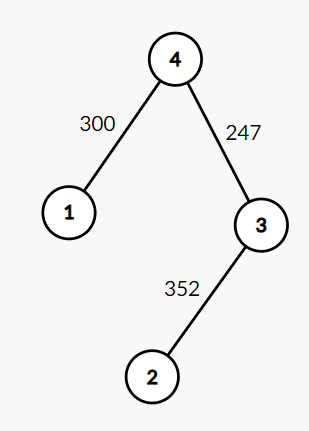
\includegraphics{graph.PNG}  
\end{center}

Bisa dilihat, negara Arkavnesia memiliki ibukota di kota ke-3.

\begin{enumerate}    
    \setlength\itemsep{0pt}
    \item   Kota yang harus dilalui perwakilan kota ke - 1 adalah 1, 2, dan 3.\\
            Harga minimum cokelat adalah min($A_1, A_2, A_3$) = $A_3$
    \item   Kota yang harus dilalui perwakilan kota ke - 2 adalah  2 dan 3.\\
            Harga minimum cokelat adalah min($A_2, A_3$) = $A_3$
    \item   Kota yang harus dilalui perwakilan kota ke - 3 adalah kota 3 itu sendiri.\\
            Harga minimum cokelat adalah min($A_3$) = $A_3$
    \item   Kota yang harus dilalui perwakilan kota ke - 4 adalah 3 dan 4.\\
            Harga minimum cokelat adalah min($A_3, A_4$) = $A_4$
    \item   Kota yang harus dilalui perwakilan kota ke - 5 adalah 3, 4, dan 5.\\
            Harga minimum cokelat adalah min($A_3, A_4, A_5$) = $A_4$
\end{enumerate}

\end{document}